%================ch3======================================
\chapter{Analysing the data}\label{ch:ch3}

\section{Radial Distribution of Stars}
The radial distributions were calculated for each cluster individually for each track. The mean shift algorithm was used to find the center of the clusters. 

\subsection{Mean Shift Algorithm}
The mean shift algorithm is an unsupervised, non-parametric, clustering algorithm. It iteratively shifts points towards the highest density of data points - cluster centers - and classifies them accordingly. It doesn't make any assumption about the model like K-means or Gaussian mixture models. The \lstinline{scikit-learn}\citep{scikit-learn} implementation was used. The model takes in a parameter - bandwidth. This bandwidth is used in the RBF kernel for the algorithm. This parameter defines how many clusters will be there in the data. Setting a relatively high value for this makes sure there is only one cluster in the data. 

\subsection{Plotting the Distributions}
The radial distance from the cluster center is calculated for every star in the cluster. The radial distance was plotted against the number of stars under that distance for a single track and a binary track. 

\begin{figure}[H]
\centering
\begin{subfigure}[b]{0.45\textwidth}
  \centering
  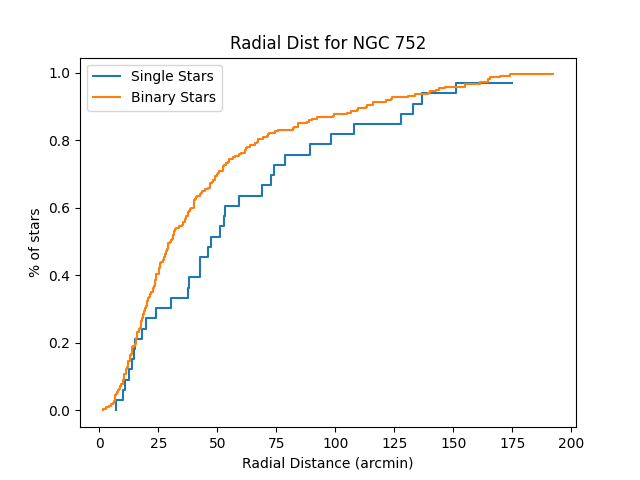
\includegraphics[width=\textwidth]{NGC 752_rad.png}
  \caption{NGC 752}
  \label{fig:im4}
 \end{subfigure}
~
\begin{subfigure}[b]{0.45\textwidth}
  \centering
  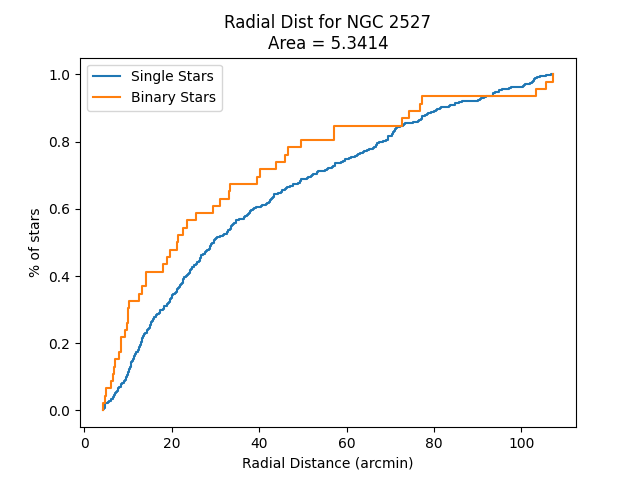
\includegraphics[width=\textwidth]{NGC 2527_rad.png}
  \caption{NGC 2527}
  \label{fig:im5}
\end{subfigure}
\caption{Radial Distribution for Star Clusters}
\label{fig:sim1}
\end{figure}

\section{King's Profile}

